\section{Implementation, Integration and Test Plan}
\subsection{Overview}
\vspace{0.5cm}
This section will discuss the implementation, integration and testing of the CLup application. The section aims to prevent any setbacks entailing changes on the project once started its development and do multiple tasks twice.\\
\\
We all make mistakes. Some of those mistakes are not important, but some are expensive, so the phase of verification and validation takes an important role. Thus, we try to find as many as bugs possible until the release day.

\subsection{Implementation Plan}
\vspace{0.5cm}

First of all, it is important to divide the project into smaller components in order to have more concrete goals that help keep the developers’ motivation high and make a straightforward development of the project. Therefore, we will divide the project in different components, starting from the ones that are responsible of the basic features and going on until the end, where we will develop the most specific ones. It is not a new method, because it has been studied during this course and it is referred to as ‘bottom-up’ strategy. This method will help providing a better integration of the project tier-by-tier and make different tests of the behaviour of the application before it ends.\\ \\
In the bottom-up approach, the implementation must start from the lower components up to the top because in this approach the implementation is gradual. In the design, there are some components that rely on other components. Thus, it's better first start implementing with the component that other components use it.\\ \\
The first step could be implementing the DB manager which is the component implementing all methods that allow to access to the Database and perform queries and updates on it.\\ \\
After that we could implement the access manager because it is impossible to implement any other component without users. then we will implement the shop manager because in our application there are two important object one of them is User and the other is the Shop. If you think in wider view, you see we want to assign some users to some shops.\\ \\
Two important service we use are Notification manager and Map manager this two components are connected to external components of our system so it's good to implement them at this stage.\\ \\
No we could implement the book manager. At this stage, we could slightly see how our application works and books, after we test this part we implement ticket handler so you could see the ticket and generate them. After the ticket handler is good to implement the estimator. estimator is one of the hard components in this application because, it must estimate user behaviors and it must estimate user arrival time and send proper notification to notification manager.\\ \\
The Redirector and Web server are implemented at the end its role is to dispatch messages coming from the client to the different parts of the system.\\
The implementation of the UserMobileApp and the TicketMachine, as just said, could be done in parallel with that of the components described before.

\subsection{Integration Strategy}
\vspace{0.5cm}

To implement and test the different functionalities of the system a bottom-up approach has been used. The following diagrams describe how the process of implementation and integration testing takes place, according to a bottom-up approach. \\

\begin{enumerate}
    
\item At first the AccessManager is implemented and unit tested using a driver for the components that are still under implementation. It is not a complex component, but other components rely on it to provide some services: that’s why it is implemented and tested before the others. \\
\begin{figure}[H]
  \centering
  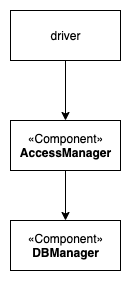
\includegraphics[width=0.2\textwidth,keepaspectratio]{images/IS/IS1.png}
\end{figure}

\item Then we implement the ShopManager, because one of the most important enitit y of our application is shop.\\
\begin{figure}[H]
  \centering
  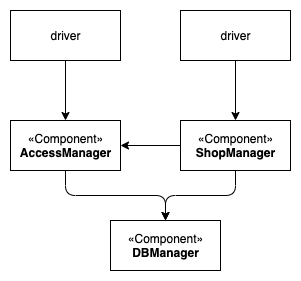
\includegraphics[width=0.4\textwidth,keepaspectratio]{images/IS/IS2.png}
\end{figure}

\item Then, to implement the functionality of notifying from the system and receiving it by the user, the NotificationMapManager is needed. However, besides the normal driver, also a stub is needed to cope with the lack of communication with the WebServer that has still to be integrated with the rest. The addition of this stub goes in contradiction with the bottom-up approach but is needed in order to proceed with the integration in the application server.\\
\begin{figure}[H]
  \centering
  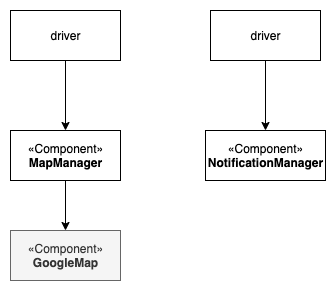
\includegraphics[width=0.4\textwidth,keepaspectratio]{images/IS/IS3.png}
\end{figure}

\item to implement the functionality of booking a slot for going to supermarket, the bookingManager is needed. . The addition of this stub goes in contradiction with the bottom-up approach but is needed in order to proceed with the integration in the application server.\\
\begin{figure}[H]
  \centering
  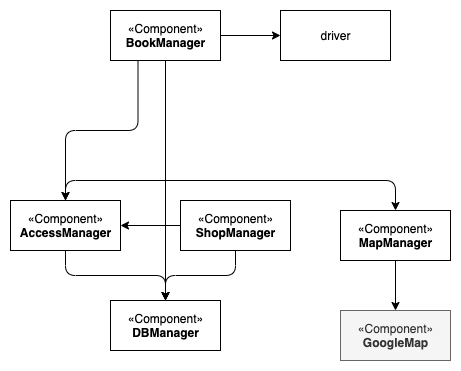
\includegraphics[width=0.5\textwidth,keepaspectratio]{images/IS/IS4.png}
\end{figure}

\item at the end of the booking we must generate the ticket, so its good to implement the ticketHandler and integerate it with other part of system.
\begin{figure}[H]
  \centering
  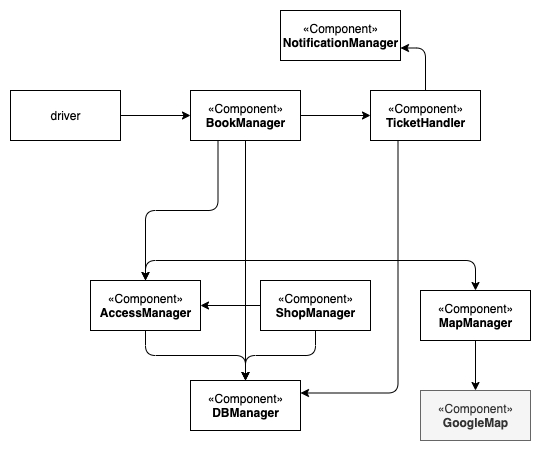
\includegraphics[width=0.6\textwidth,keepaspectratio]{images/IS/IS5.png}
\end{figure}

\item Then the Estimator is implemented, unit-tested and then integrated into the system. It is important to notice that GoogleMapsService will not be unit tested because is offered as a service from a trusted provider: it only needs to be integrated into the system through the Estimator.\\
\begin{figure}[H]
  \centering
  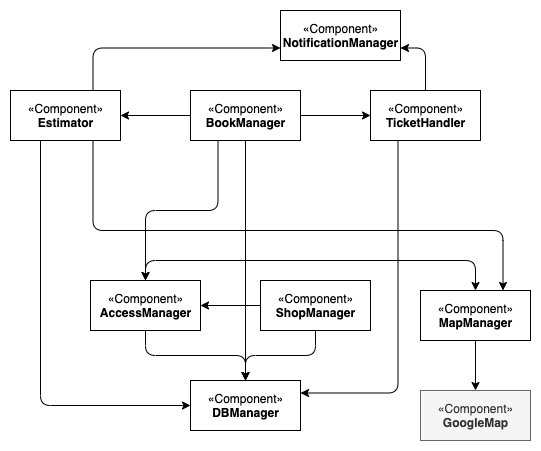
\includegraphics[width=0.6\textwidth,keepaspectratio]{images/IS/IS6.png}
\end{figure}

\item Then the different drivers are substituted by the Redirector which has to be implemented, unit-tested and integrated with the other components of the application server. its role is to allow the flow of called methods from the client to the server.\\
\begin{figure}[H]
  \centering
  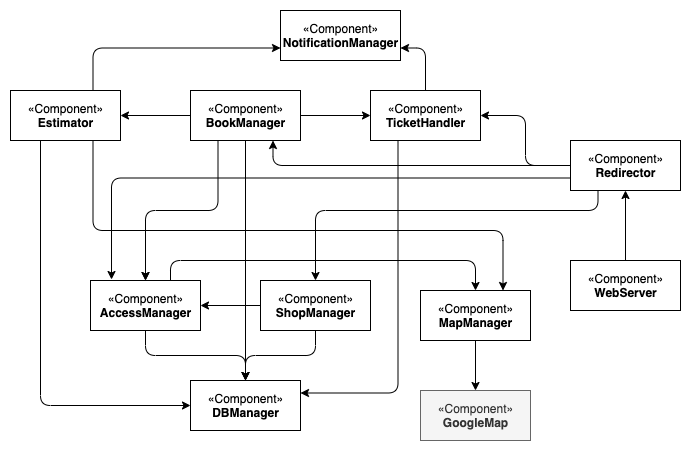
\includegraphics[width=0.8\textwidth,keepaspectratio]{images/IS/IS7.png}
\end{figure}
\end{enumerate}
